\documentclass{article}
\usepackage[paperwidth=320pt,paperheight=230pt,margin=0pt,noheadfoot]{geometry}
\usepackage{tikz}
\usetikzlibrary{calc}

\definecolor{ink}{RGB}{28,41,56}
\definecolor{axis}{RGB}{100,116,139}
\definecolor{grid}{RGB}{203,213,225}
\definecolor{curve}{RGB}{30,64,175}
\definecolor{teal}{RGB}{13,148,136}
\definecolor{tealfill}{RGB}{176,227,219}
\definecolor{orange}{RGB}{234,88,12}
\definecolor{orangefill}{RGB}{254,215,170}
\definecolor{purple}{RGB}{126,34,206}
\definecolor{yellowfill}{RGB}{254,243,199}
\definecolor{yellowedge}{RGB}{202,138,4}
\definecolor{projection}{RGB}{148,163,184}

\pagestyle{empty}
\setlength\parindent{0pt}
\setlength\topskip{0pt}
\begin{document}
\noindent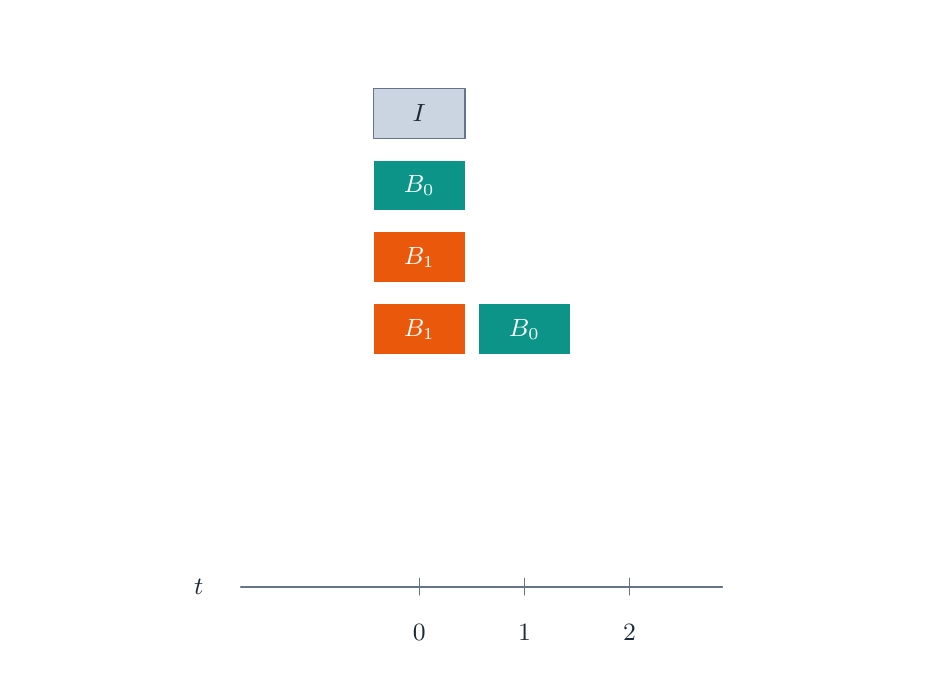
\begin{tikzpicture}[baseline=(current bounding box.north),x=1pt,y=1pt,line cap=round,line join=round]
\useasboundingbox (0,0) rectangle (320,230);
\path[fill=grid,draw=axis,line width=.45pt] (125,190) rectangle (158,208);
\node[font=\small,text=ink] at (141.5,199) {$I$};
\path[fill=teal] (125,164) rectangle (158,182);
\node[font=\small,text=white] at (141.5,173) {$B_0$};
\path[fill=orange] (125,138) rectangle (158,156);
\node[font=\small,text=white] at (141.5,147) {$B_1$};
\path[fill=orange] (125,112) rectangle (158,130);
\node[font=\small,text=white] at (141.5,121) {$B_1$};
\path[fill=teal] (163,112) rectangle (196,130);
\node[font=\small,text=white] at (179.5,121) {$B_0$};
\draw[axis,line width=.65pt] (77,28) -- (251,28);
\draw[axis,line width=.5pt] (141.5,25) -- (141.5,31);
\node[font=\small,text=ink,anchor=north] at (141.5,18) {$0$};
\draw[axis,line width=.5pt] (179.5,25) -- (179.5,31);
\node[font=\small,text=ink,anchor=north] at (179.5,18) {$1$};
\draw[axis,line width=.5pt] (217.5,25) -- (217.5,31);
\node[font=\small,text=ink,anchor=north] at (217.5,18) {$2$};
\node[font=\small,text=ink,anchor=east] at (67,28) {$t$};
\end{tikzpicture}
\end{document}
